% chktex-file 2% chktex-file 29
% chktex-file 13
\documentclass{report}
\usepackage{setspace}
\usepackage[a4paper, total={7in, 10in}]{geometry}
\usepackage[fleqn]{amsmath}
\usepackage{empheq}
\usepackage{amssymb}
\usepackage{amsthm}
\usepackage{gensymb}
\usepackage[fleqn]{cases}
\usepackage{multicol}
\usepackage{color}
\usepackage{stix}
\usepackage{chngcntr}
\usepackage{tikz}
\usepackage{enumitem}
\usepackage{pgfplots}
\usepackage{etoolbox}
\usepackage{tikz-3dplot}
\usepackage{tkz-euclide}
\usepackage{enumitem}

\def\nswe#1#2#3{#1\,$#2^\circ\,#3'$}
\graphicspath{ {./assets/} }
\usetikzlibrary{calc,matrix,arrows}
\usetikzlibrary{decorations.pathmorphing,patterns, calligraphy, perspective,backgrounds}

\counterwithout{equation}{chapter}
\setlength{\columnseprule}{1pt}
\setlength{\columnsep}{24pt}
\setcounter{chapter}{16}
\hfuzz=100pt

\newcommand{\pgfplotsdrawaxis}{\pgfplots@draw@axis}
\makeatother
\pgfplotsset{only axis on top/.style={axis on top=false, after end axis/.code={
                    \pgfplotsset{axis line style=opaque, ticklabel style=opaque, tick style={thick,opaque},
                        grid=none}\pgfplotsdrawaxis}}}

\newtheorem{theorem}{Theorem}

\begin{document}

\newcommand{\sol}[1]{

    \noindent \textbf{Sol.}
}
\newcommand{\prooff}[1]{

    \noindent \textbf{Proof.}
}
\newcommand\m[1]{\begin{pmatrix}#1\end{pmatrix}}
\newcommand\vm[1]{\begin{vmatrix}#1\end{vmatrix}}
\newenvironment{amatrix}[1]{%
    \left(\begin{array}{@{}*{#1}{c}|c@{}}
        }{%
    \end{array}\right)
}
\newenvironment{cequation}{
    \makeatletter
    \setbool{@fleqn}{false}
    \makeatother
    \begin{equation*}
        }{\end{equation*}}

\begin{titlepage}
    \raggedleft{}
    \rule{1pt}{\textheight}
    \hspace{0.02\textwidth}
    \parbox[b]{0.75\textwidth}{

    {\Huge\bfseries Solution Book of \\[0.5\baselineskip] Mathematic}\\[2\baselineskip]
    {\large\textit{Ssnior 2 Part I}}\\[4\baselineskip]
    {\Large\textsc{MELVIN CHIA}}

    \vspace{0.5\textheight}

    {\noindent Written on 9 October 2022}\\[\baselineskip]
    }

\end{titlepage}

\doublespacing{}
\tableofcontents
\singlespacing{}
\newpage

\begin{multicols}{2}
    \begin{enumerate}
        \item The diagram below shows a roof, $HK$ is the ridge of the roof, its edges $HA$,
              $HD$, $KB$, $KC$ are euqal in length. Both of the planes $HAD$ and $KBC$ form a
              $44^o$ angle with plane $ABCD$. Given that $S$ and $T$ are the midpoints of
              $BC$ and $AD$ respectively. Find:
              \begin{center}
                  \includegraphics[scale=0.9]{roof}
              \end{center}
              \begin{enumerate}
                  \item The distance from line $HK$ to plane $ABCD$. \sol{}

                        Let the foot point of $K$ on plane $ABCD$ be $P$.
                        \begin{flalign*}
                            \text{In } \Delta KPS, \sin{\angle{KSP}} & = \frac{KP}{KS}   \\
                            \sin{44^\circ}                           & = \frac{KP}{2}    \\
                            KP                                       & = 2\sin{44^\circ} \\
                                                                     & \approx 1.39m
                        \end{flalign*}

                  \item The length of $HK$. \sol{}
                        \begin{flalign*}
                            \cos{\angle{KSP}} & = \frac{PS}{KS}   \\
                            \cos{44^\circ}    & = \frac{PS}{2}    \\
                            PS                & = 2\cos{44^\circ} \\
                                              & \approx 1.44m     \\
                            HK                & \approx 12 - 2PS  \\
                                              & \approx 12 - 2.88 \\
                                              & \approx 9.12m
                        \end{flalign*}

                  \item The angle formed by line $HA$ and plane $ABCD$. \sol{}

                        Let the foot point of $H$ on plane $ABCD$ be $Q$.
                        \begin{flalign*}
                            HA & = \sqrt{HT^2 + AT^2} \\
                               & = \sqrt{2^2 + 4.5^2} \\
                               & = \sqrt{24.25}cm     \\
                        \end{flalign*}
                        The angle formed by line $HA$ and plane $ABCD$ is $\angle{HAQ}$.
                        \begin{center}
                            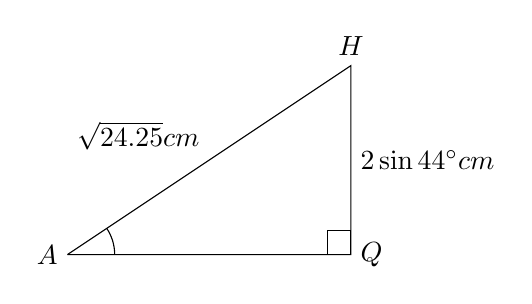
\begin{tikzpicture}[scale=1.2]%,cap=round,>=latex]

                                \coordinate [label=left:$A$] (A) at (-1.5cm,-1.cm);
                                \coordinate [label=right:$Q$] (C) at (1.5cm,-1.0cm);
                                \coordinate [label=above:$H$] (B) at (1.5cm,1.0cm);
                                \draw (A) -- node[midway,above left] {$\sqrt{24.25}cm$} (B) -- node[midway, right] {$2\sin{44^\circ}cm$} (C) -- node[below] {} (A);

                                \draw (1.25cm,-1.0cm) rectangle (1.5cm,-0.75cm);
                                \tkzMarkAngle[size=0.5cm,color=black,mark=](C,A,B)
                            \end{tikzpicture}
                        \end{center}
                        \begin{flalign*}
                            \sin{\angle{HAQ}} & = \frac{HQ}{HA}                        \\
                            \sin{\angle{HAQ}} & = \frac{2\sin{44^\circ}}{\sqrt{24.25}} \\
                            \angle{HAQ}       & \approx 16.38^\circ
                        \end{flalign*}
              \end{enumerate}

        \item The length, width and height of a hall are $20m$, $15m$, and $4m$ respectively.
              Find:
              \begin{enumerate}
                  \item The length of the diagonal of the hall.
                  \item The angle formed by the diagonal and the floor of the hall.
              \end{enumerate}
              \begin{center}
                  \includegraphics[scale=0.9]{hall}
              \end{center}
        \item In the diagram below, $ABCD$ represents a rectangular plank with length and
              width of $60cm$ and $36cm$ respectively, its base $BC$ is on the ground and the
              top of it lies on the wall. Assume that the distance between $BC$ and the
              corner of the wall is $12cm$, find the angle formed by the diagonal $BD$ of the
              plank and the ground.
              \begin{center}
                  \includegraphics[scale=0.9]{wall}
              \end{center}
    \end{enumerate}
\end{multicols}
\end{document}